\setlength{\epigraphrule}{0\p@}
\setlength{\epigraphwidth}{.7\textwidth}
\epigraph{\textit{"The embryo in the course of development generally rises in organisation (...) I am aware that it is hardly possible to define clearly what is meant by the organisation being higher or lower. But no one probably will dispute that the butterfly is higher than the caterpillar."}}{Charles Darwin 1859}

In this section, I will talk about the increase in complexity during embryonic development.
I will first try to explain different existing definitions of organismic complexity.
Then, I will explore the relationship between complexity in evolution and development, and discuss the possibility of a trend in terms of complexity increase.


\subsection{Different definitions of complexity}


\subsubsection{Complexity in informational terms}

The use of informational terms (e.g., transcription, translation and code) in biology are widespread, specially in molecular biology \citep{Smith2000,yockey2005information}
More than just the use of informational terms in biology, information theory concepts like Shannon's entropy and mutual information have been used as a proxy to measure complexity.
In the following paragraphs, I will briefly describe briefly these concepts and provide some examples of their use to address biological complexity.

\paragraph{Shannon's entropy}

Shannon's entropy is a measure of uncertainty. Given a set of $n$ possible events whose probabilities of occurrence are $p_{1}, p_{2}...,p_{n}$, Shannon's entropy ($H$) can be defined as:

$$H = -\sum_{i=1}^{n} p_{i} \log p_{i}$$

For a given $n$, the maximum $H$ is equal to $\log n$ when all the events have the same probability (i.e., $\frac{1}{n}$) \citep{Shannon1948}. The logarithmic base of 2 corresponds to binary digits units, or \textit{bits}.

This can be illustrated measuring $H$ for a nucleotide position in the DNA sequence. As in principle, each DNA site can take four possible values (A, T, G or C), its maximal entropy can be calculated as:

$$H_{max} = -\sum_{i=A,T,G,C}^{} p(i) \log_{2} p(i) = \log_{2} 4 = 2 bits $$

Cristoph Adami have used Shannon's entropy to define a "physical complexity" measure, that refers to the "amount of information that is stored in that sequence about a particular environment" \citep{Adami2002}.
%
More specifically, Adami's complexity measure compares the maximum entropy of a specific DNA sequence with the "actual" entropy based on the actual probabilities $p_{j}(i)$ for each position $j$ in the sequence. Given a pool of N sequences, $p_{j}(i)$ is estimated by counting the number $n_{j}(i)$  of occurrences of nucleotide $i$ at position $j$, so that $p_{j}(i)=n_{j}(i)/N$ (for all positions $j =1,...,L$ of the sequence with length $L$) \citep{Adami2000}. 
The information content of a DNA sequence is then $I = H_{max} - H $  where:

$$H = -\sum_{j=1}^{L} \sum_{i=A,T,G,C}^{} p_{j}(i) \log_{2} p_{j}(i) $$

Adami assumes that if a sequence has not been under selective pressures each position in the sequence would have any of the four nucleotides with the same probabilities, so the actual entropy would be equal to the maximal, and consequently the information would be zero \citep{Adami2002}. 
%In the presence of selection, the probabilities of finding a particular nucleotide in a specific size would be non-random, giving a positive value of the information. He finally proposes that if natural selection is efficient "physical complexity" will increase and that it would decrease if is not \citep{Adami2002a}.
He also considers that the "physical complexity" would serve as a good predictor of functional complexity \citep{Adami2004}. 
His information measure is related to the degree of conservation of a given sequence, which in the case of protein sequence has indeed been used to identify its functionality \citep{Casari1995,Kellis2003,Hannenhalli2000}.


\paragraph{Mutual information}

A concept related to Shannon's entropy that has been used in biological sciences is the concept of mutual information. Mutual information is a measure of the information in one variable about another. It is measured using the "conditional entropy" concept (the entropy of a variable $Y$ given that $X$ is known)  introduced also by \citet{Shannon1948}.
The mutual information $I(X;Y)$ of variables $X$ and $Y$ can be expressed as:
 
 $$I(X;Y) = H(X) - H(X|Y)$$

where $H(X)$ is the Shannon's entropy of $X$ and $H(X|Y)$ is the conditional entropy of $X$ given $Y$. As Shannon's entropy, the conditional entropy is a measure of uncertainty. In this case, $H(X|Y)$ measures how uncertain we are of $Y$ on the average when we know $X$ \citep{Shannon1948}.

Therefore, mutual information measures how much information of one variable is contained in the other. It can also be though as a similarity measure \citep{yockey2005information}, as if $X$ is identical to $Y$, the information of knowing $X$ determines the value of $Y$.
Some decades ago, there were great expectations on the use of informational measures to predict some features of an organism based on its DNA or protein sequences. For example, it was thought that the DNA sequence of a coding gene would determine not only the sequence of a protein, but also its 3D folded structure \citep{Anfinsen1973}.
However, it is nowadays clear that other factors like post-translational modifications and the physico-chemical environment of the protein affect its structure \citep{Kang2009} and that the DNA sequence is not sufficient to predict it.

This lack of correspondence between DNA and proteins have restrict the application of the mutual information as a similarity measure that compares DNA \citep{Lichtenstein2015} or protein sequences \citep{Gloor2005} separately.

However it has been proved useful to analyse different aspects of these molecular sequences, the informational approach has not been successfully applied to higher organisation levels (i.e., cells, tissues, organism) \citep{Longo2012}. It has also been noted \citep{Jaeger2014devmech} that the use of the informational approach is not appropriate to the study of development, simply because Shannon's information can not 
increase while it is transmitted. If applied to development, it would imply that the amount of information (or complexity) of the egg and the adult remain constant \citep{Jaeger2014devmech}, which contradicts the generalized notion that the complexity increases during embryogenesis.
 

\subsubsection{Computational metaphors}
Many authors have used computational analogies to define development \citep{Apter1965,monod2012cytodifferentiation,mayr1997evolution,Davidson2001}. Eric H. Davidson used the gene regulatory network (GRN) concept and a computational metaphor to explain development (and evolution). A GRN consists of DNA cis-regulatory elements, i.e., the regions in the vicinity of each gene which contain the specific sequence motifs at which those regulatory proteins which affect its expression bind; plus the set of genes which encode these specific regulatory proteins (i.e., transcription factors) \citep{Davidson2001}. For Davidson, development is then the outcome of spatial and temporal series of differential gene expression, that is controlled by a "regulatory program" (the GRN) built into the DNA.
	\nomenclature{GRN}{Gene Regulatory Network}

%To illustrate how the complexity of a regulatory network or "program" can increase in evolution (but a similar case could be said for development), Davidson describes an imaginary example:
%an early evolutionary state consists of a small gene battery (set of functionally linked genes expressed in concert) encoding proteins used for some differentiated cell type, which is activated by a small number of genes encoding transcription factors. The network activating the gene battery is itself controlled by a single upstream gene.
%In subsequent evolutionary states, the whole structure is said to become more complex as: the battery of genes is now used in some pattern formation system, new batteries of genes appear, new regulatory genes and new \textit{cis}-regulatory regions are introduced  \citep{Davidson2001}.
A computational program, that is part of a computer system, contains a set of instructions that performs a specific task. The computer program needs a hardware, the set of physical objects that compose the computational system and where the computational program can be stored and execute.
If the cell is considered as a computer system with the GRN as the computer program, then the hardware would be all the components of the cell including the genomic and cell structure and all the molecules present in the cell.
However, in contrast to a computer system, the separation between the program and the hardware is not clear in a cell. The "genetic program" is affected by the components present in the cell ("hardware"), which in turn changes depending on the program \citep{susan2000ontogeny,Jaeger2014devmech}.
%
%There are also important critiques of this informational approach. First, using an informational analogy to describe development implies the distinction between a "hardware" and a "software".
%The "hardware" would consist of the genome structure, regulatory components, cells, organs, etc., and the "software" would be the GRNs or the set of instructions that directs the performance of specific operations.
%For biological systems, this distinction is misleading, as there are recurrent feedback between its "hardware" and "software", so that the structure of development processes change through development \citep{susan2000ontogeny,Salazar-Ciudad2009,Jaeger2014devmech}.

Using again the computational metaphor, Davidson considered that these programs of gene expression, which are "installed and executed" as the embryo develops, could serve as a metric of complexity \citep{Davidson2001}. For illustrating his point Davidson describes an imaginary example of a GRN that increases its complexity in evolution: first, there is a set of downstream genes activated by a small network of TFs (each of them with only one \textit{cis}-regulatory element), which in turn is controlled by a single upstream TF; then, TFs of the network gain cis-regulatory elements (so the circuitry is more intricate) and newly recruited intermediate regulatory TFs activate a different set of down-stream genes. Otherwise, the initial set of downstream genes is still controlled by the single upstream TF \citep{Davidson2001}.
   
Thus, in Davidson example, a small hierarchical network changes so that an additional layer is gained (intermediate TF) and the topology of the network changes: instead of one outcome (the initial set of downstream genes), now two outcomes are possible (with the additional set of downstream genes activated by the new intermediate TF).
Even when in his example it would seem easy to discern a simple GRN from a complex one just from its topology, the high intricacy of real biological GRN would make their distinction (at least by visual inspection) a very difficult task.

%an early evolutionary state consists of a small gene battery (set of functionally linked genes expressed in concert) encoding proteins used for some differentiated cell type, which is activated by a small number of genes encoding transcription factors. The network activating the gene battery is itself controlled by a single upstream gene.
%In subsequent evolutionary states, the whole structure is said to become more complex as: the battery of genes is now used in some pattern formation system, new batteries of genes appear, new regulatory genes and new \textit{cis}-regulatory regions are introduced
%
%
%%%%%%%%%%%%%%%%%%%%%%%%%%%%%%%%%%%%%%%%%%%%%%%%%%%%%%%%%%%%%%%%%%%%%%%%%%%%%%%%%%%%%%
%\begin{figure}[h]
%  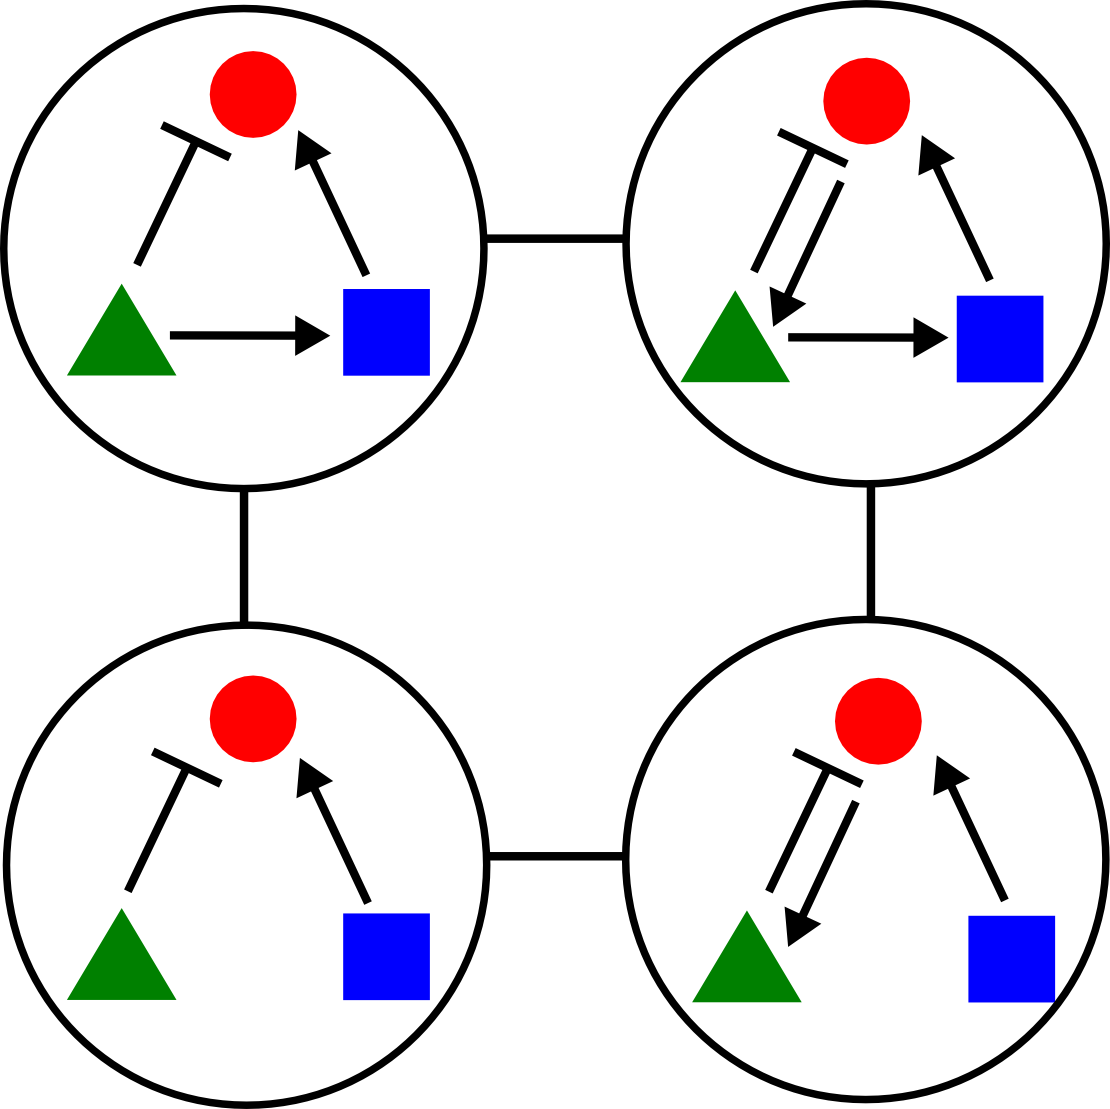
\includegraphics[width=5cm]{./Images/GRNs.png}
%  \centering
%  \caption{
%  Some GRNs . Cotterel and Harpe calculated... \citep{Cotterell2010}
% }
%  \label{fig:GRNs}
%\end{figure}
%%%%%%%%%%%%%%%%%%%%%%%%%%%%%%%%%%%%%%%%%%%%%%%%%%%%%%%%%%%%%%%%%%%%%%%%%%%%%%%%%%%%%%
%
%\subsubsection{Complexity in terms of dynamical systems theory}
%
%Dynamical systems theory (DST) has been proposed as an alternative to analyse complex GRNs. DST is branch of mathematics used to describe complex systems usually with differential or difference equations. 
%In developmental biology, DST has been used to identify the set of networks that can produce a certain output. 
%For example, Cotterel and Sharpe defined all the possible regulatory topologies of a simple three-gene GRN (in which each gene can activate or inhibit the expression of any gene including its own), and then identified the subset of network capable of the formation of a single stripe of gene expression in a one-dimensional cell array. They determined that only 471 of the possible 3379 topologies were capable of such task \citep{Cotterell2010}.
%
%
%Estimating the combinatorial possibilities of a small set of regulatory genes, considering that each gene can regulate (whether positively or negatively) more than one gene's expression in addition to its own, could result in an astronomic number of possible gene topologies (see Figure \ref{fig:GRNs}).
%Also feedback effects and non-linear regulation of gene expression make the prediction of changes in regulatory states hard or even impossible to predict \citep{Jaeger2014devmech}.
%
%To overcome this limitations, some authors have propose to use dynamical systems theory, which deals with a complex system with many interacting components (a dynamical system), by representing its state as a point in a multidimensional space \citep{Alberch1991,ForgacsandStuartA.Newman.2005,Jaeger2014devmech}. 
%To illustrate this we could think of a specific cell type, with \textit{n} number of genes, which its cell state depends on the expression of each of the genes.
%The simpler case we could imagine would be a cell with only two genes. In this case, the cell would be in a two-dimensional "state space" (also called "phase space").
%
%Importantly, the dynamical system is governed by the relations between its components \citep{ForgacsandStuartA.Newman.2005}. In our example the relations would be represented by the interaction between genes, namely the gene regulatory network (GRN). 
%If in our example the expression level of one gene is affected by the expression level of the other gene, the system will not stay in any particular state, but it will change until it reaches a "stable steady state", in which the level of both genes are at equilibrium. 
%Given a specific GRN, the number of stable states would represent the possible differentiation states a cell can achieve (REF Slack book)
%
%Many modifications of the GRN would not have consequences in the ultimate differentiation state, as it will converge to the same "attractor" point.
%However, some modifications (or mutations) could produce a change in the "state space" leading to the formation of a new stable state (i.e., a new cell type).
%So within the framework of the dynamical systems theory, and keeping the number of cell types as our measure of complexity, there would be an increase in complexity when a mutation would change the gene regulatory machinery so that a new stable steady state is formed.


\subsubsection{McShea's view of complexity}

Daniel W. McShea has provided useful definitions of biological complexity. One of his definitions is: "complexity of an organism is the amount of differentiation among its parts or, where variation is discontinuous, the number of part types" \citep{McShea1996,McShea2015}.
This definition can be used at different hierarchical levels of biological organization, e.g., tissues, cells, genes.
Indeed, a measure of morphological complexity that has been favoured by some authors 
%(perhaps because of its intuitiveness), 
is the number of cell types that compose an organism 
	\citep{Valentine1994,Bell1997,Bonner2004}.
Importantly, with this definition, complexity at different levels are not necessarily correlated.

%These "parts" might be body segments (e.g., of an insect) or genes.
%It is evident that these definitions are problematic.
%It is doubtful to say that some centipede is more complex than a beetle, just based in the different number of segments they have.
This lack of correspondence at different levels using "the number of part types" its evident comparing the number of genes with the number of cell types. Before the release of the first eukaryotic genome sequences, it was expected that the number of genes would correlate with an intuitive perception of organismal complexity, ranking complexity as yeast $<$ nematodes $<$ flies $<$ humans \citep{Hahn2002} (this intuitive notion of complexity correlates with the number of cell types in metazoans; \citealp{Valentine1994}). However, this expectation was proved to be wrong and this lack of correlation between "intuitive complexity" and genes number was called the "G-value paradox" \citep{Hahn2002}.
%This is related with the already acknowledged lack of correlation between the number of coding-genes and morphological complexity, 
%This lack of correspondence, 
%sometimes referred as the "G-value paradox"
%	\citep{Hahn2002}.
%Some decades ago, there was the expectation that the morphological complexity should correlate with the number of genes in an organism. 
%With the release of the first eukaryotic genome sequences, such correspondence was not observed.
Before that, the lack of correspondence between genome size and organism complexity (using again an intuitive notion of complexity),  or "C-value paradox", was also noted.


McShea also makes the distinction between "object complexity" that refers to the number of parts of a system and "process complexity" that refers to the interaction among parts in a system \citep{McShea1996}.
%An alternative definition of complexity includes not only the "number of parts" but also the "interaction among parts" 
%	\citep{McShea1996,Arthur2010}.
This could be illustrated with the number genes (object complexity) and the number of gene-gene interactions (process complexity). Gene-gene interactions would refer to the regulation of a gene expression by the binding of another gene product (transcription factor) to its promoter region.
Using this definition, two different organisms would have the same object complexity if they have the same number of genes, but one would have a higher process complexity it has more gene-gene interactions than the other.


%%%%%%%%%%%%%%%%%%%%%%%%%%%%%%%%%%%%%%%%%%%%%%%%%%%%%%%%%%%%%%%%%%%%%%%%%%%%%%%%%%%%%%%%%%%%%%%%%%%%%%%%%%%%%%%%%%%%%
\subsection{Complexity Increase in Development}

The increase in complexity in an organism during embryogenesis is probably one of the most intuitive processes of animal development.

It is commonly seen even as one of its defining characteristics.
Eric H. Davidson described the progressive increase in complexity as the "essence" of development \citep{Davidson2001}. Despite of the widely accepted view of complexity increase in development, there is no consensus of how to define it, much less on how to quantify it \citep{susan2000ontogeny}.

%One of the most accepted definitions of complexity is the number of cell types in an organism \citep{Valentine1994,McShea1996,Bell1997,Bonner2004,Arthur2010}.

Using the number of cell types, the increase of complexity during development is self-evident: in vertebrates, the embryo begins with one cell type (the zygote) and concludes with more than 200 cell types \citep{Alberts1994}. 

%Using the number of cell types again as a proxy of morphological complexity, it can be said that during metazoan development, complexity increases as the zygote divides and differentiates into an adult with multiple cell types. 

This definition of complexity is not exempt of complications, as there is no clear criteria of how to define a cell type or how to determine when a new cell type has formed during development. 
%For example, it could be that at the morphological level a cell seems to be undifferentiated, but when isolating it from its neighbour cells, it differentiates in an autonomous way into a specific cell type, suggesting that the cell fate was already determined without the necessity of further interactions with other cells.
%
In addition, this definition does not take into account that embryos do not only get more cell types, but they also get organized in specific patterns in space and time in the embryo, which also could be considered as an increase in complexity over developmental time.

The notion of an increase in complexity during embryogenesis is tightly related to the concept of embryo compartmentalization.


%%%%%%%%%%%%%%%%%%%%%%%%%%%%%%%%%%%%%%%%%%%%%%%%%%%%%%%%%%%%%%%%%%%%%%%%%%%%%%%%%%%%%
\clearpage

\setcounter{figure}{2}% Modify counter of figure so it maches the order, as here im not using \begin{figure}

\begin{mdframed}[style=boxstyle,frametitle={Box1. On the relationship between the increase of complexity in Evolution and Development}]\label{Box1:Evo_complexity}

The connection between the increase in complexity during development and evolutionary time it has been largely discussed.
Haeckel was one of the first who made explicit hypotheses about the connection between the development and evolutionary patterns in his "Biogenetic Law" (see section X).

This implies that the increase in complexity we see during development is a reflection of a similar increase in complexity that has occurred through evolution.

Early views of evolution saw the increase in complexity as inexorable, with all the species descending from simpler ancestral forms \citep{lamarck1809zoo,haeckel1874menschen}, and with the human species as the latest and more perfect product of the evolution of animals \citep{haeckel1874menschen}.


Recent views recognize that complexity of can increase or decrease in a lineage.
Using the number of cell-types as complexity measure, there are clear examples of taxa that have decreased their complexity over time, specially in parasites \citep{Canning2003,Arthur2010} (although morphological simplification can not be considered universal in parasitic taxa \citealp{poulin2011evolutionary}). Therefore, it seems that there is no unique trend to increase the complexity over time. Therefore, the complexity of a specific lineage might decrease, increase or stay the same (see Figure \ref{boxfigure}.
%%%%%%%%%%%%%%%%%%%%%%%%%%%%%%%%%%%%%%%%
\par
{\centering
  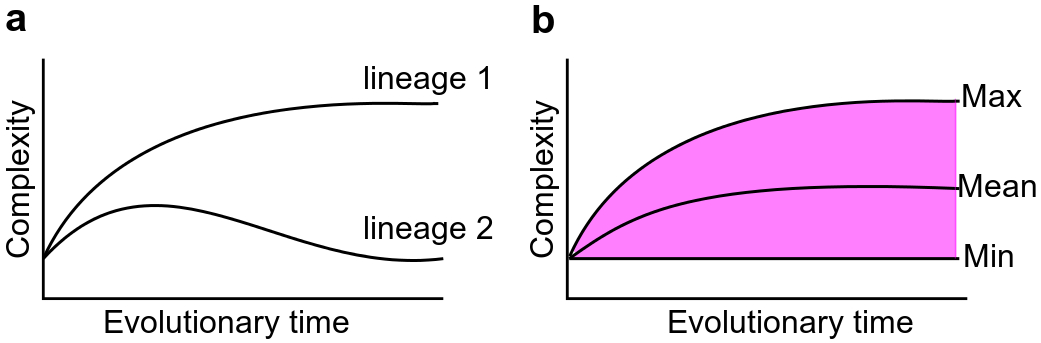
\includegraphics[width=0.8\textwidth]{./Images/complexity_min.jpeg}
  \centering
  \captionof{figure}{Two lineages with different complexity change through their evolutionary trajectories.
  b) Representation of the minimum, mean and maximum complexity of many lineages over evolutionary time in which the minimum stay constant while the mean and maximum increase.
Redrawn from \citep{Arthur2010}.}
\label{boxfigure}
}
\par
%%%%%%%%%%%%%%%%%%%%%%%%%%%

If we consider unicellularity as the minimum complexity, it can be said that complexity has remained more or less constant in evolution, as unicellular organisms like bacteria, have been present from 3.5 billion years.

If we look at maximum complexity a trend for increasing complexity would be apparent, as the initial complexity would have increased with the appearance of simple multicellular organisms (only few cell types) and would have further increase until the appearance of organisms composed of hundreds of cell types.

It is important to notice that this apparent trend towards increasing complexity does not necessarily imply that it has been selected for \citep{McShea2015}.

If complexity would follow a random walk scenario starting from unicellular organisms (in a random walk the mean distance of a point after $n$ time steps is $\sqrt[2]{n}$), the mean and maximum would show a trend towards increasing complexity \ref{boxfigure} given that there is a minimum complexity requirement (it is not possible to have less than one cell) \citep{gould1996fullhouse}.

\end{mdframed}
%%%%%%%%%%%%%%%%%%%%%%%%%%%%%%%%%%%%%%%%%%%%%%%%%%%%%%%%%%%%%%%%%%%%%%%%%%%%%%%%%%%%%

\subsubsection{Compartmentalization in development}

In here, I will refer to compartmentalization as the subdivision of the embryo in different parts (or compartments) during development. 
How the different parts of the embryo can be defined based on the cell-phenotype or gene expression profile.

It is usually considered that the earliest compartments that are formed in the embryo define the main body axis, i.e., the anterior/posterior (A/P) and dorsal/ventral (D/V) axes.
	\nomenclature{A/P}{anterior/posterior}
	\nomenclature{D/V}{dorsal/ventral}
Later on, smaller compartments of the embryo would be formed, e.g, limbs, eyes or internal organs. In this manner as development proceeds, it is expected that spatial compartments would be progressively specified at an increasing finer resolution \citep{Davidson2001}.
%However, the definition of pattern is different from the compartments one, in that the a pattern transformation does not necessarily involves changes in gene expression. A new pattern could be formed by a morphogenetic process, e.g., migration.
%\hfill \break
%This progressively compartmentalization is expected to be reflected at the level of gene expression: genes would be expressed ubiquitously at very early development, then some would be expressed in large regions in the embryo defining the main embryo axes and in later developmental stages some genes would be expressed in cell-specific or tissue-specific manner. 
Furthermore, the increasing compartmentalization of the embryo during development can be conceptualized as the progressive spatial restriction of gene expression to subsequently smaller regions in the embryo.
Sean Carroll defines this process\citep{Carroll2001} as:
%%%%%%%%%%%%%%%%%%%%%%%%%%%%%%%%%%%%%%%%%%%%%%%%%%%%%%%%%%%%%%%%%%%%%%%%%%%%%%%%%%%%
\begin{enumerate}
\item In early development, genes have a broad expression in the embryo and define the main axes of the body.
\item Later, genes define smaller compartments like organs and appendages (field-specific selector genes).
\item Finally, genes become expressed in specific cell types like muscle and neural cells (cell-type specific selector genes). 
\end{enumerate}
%%%%%%%%%%%%%%%%%%%%%%%%%%%%%%%%%%%%%%%%%%%%%%%%%%%%%%%%%%%%%%%%%%%%%%%%%%%%%%%%%%%%
It is important to note that this would imply that, in general, the area of expression of a gene in the embryo would decrease during development (relative to the area of the whole embryo).

A well known definition of developmental compartment was proposed by \citet{Garcia-Bellido1973}. They defined compartments as differentiated populations of cells (at the gene expression level) that do not intermix between them that are formed from initially homogeneous contiguous cells. 
The definition used in here is related to the one of Garcia Bell\'{i}do et al., but in contrast to it, does not rely on the identification of a boundary formation between different cell populations that would prevent cell mixing between them.
%\citet{Garcia-Bellido1973} proposed this concept after an experiment using clonal analysis, in which they found that different parts of the fly wing were subsequently determined in the imaginal disc by the formation of differentiated populations of cells that do not intermix between them.
%They demonstrated that the imaginal disc is initially divided in two compartments: anterior and posterior that subdivide into smaller compartments that pre-define specific parts of the adult wing.  It was later proposed that the compartmentalisation was specified by a genetic code like a ZIP address \citep{Garcia-Bellido1979}.

%\subsubsection{Developmental pattern}
%A developmental pattern can be defined as the specific distribution of cell types in a specific temporal window of embryonic development \citep{Salazar-Ciudad2004}. 
%Therefore, development can be conceptualized as the continuous transformation of one pattern into another.
%This relates to the compartments definition, as the earliest pattern transformations usually establish the main axis or "compartments" of the embryo. For example, the anterior/posterior (A/P) and dorsal/ventral (D/V) axes in the fruit fly.
%	\nomenclature{A/P}{anterior/posterior}
%	\nomenclature{D/V}{dorsal/ventral}
%Later pattern transformations would define smaller compartments of the embryo, e.g, limbs, fingers  or internal organs.
%However, the definition of pattern is different from the compartments one, in that the a pattern transformation does not necessarily involves changes in gene expression. A new pattern could be formed by a morphogenetic process, e.g., migration.
%\hfill \break
%As development proceeds, spatial compartments are progressively specified at an increasing finer resolution \citep{Davidson2001}.
%Thus, a great proportion of pattern transformation involve the partition of specific embryo compartments into smaller sub-compartments.
%
%The compartmentalization of the embryo can be considered then an intrinsic property of development and could be used as a proxy of complexity.


\subsubsection{Complexity at the molecular level}

For some authors, the increase in complexity in an organism during development (reflected by the increase of number of cell types), should be associated with an underlying complexity at the molecular level \citep{Davidson2001,Arthur2010}, following the reasoning that:
%If we consider again the number of cells as the complexity measure, it could be expected that the increase in complexity over developmental time should be associated with an underlying increase in complexity at the molecular level \citep{Arthur2010}, following the reasoning that:

%%%%%%%%%%%%%%%%%%%%%%%%%%%%%%%%%%%%%%%%%%%%%%%%%%%%%%%%%%%%%%%%%%%%%%%%%%%%%%%%%%%%
\begin{enumerate}
\item In development, complexity increases with time as new cell types form.
\item Different cell-types are characterized by the differential expression of genes.
%\item Therefore, the more cell-types an organism is formed of, the more different combinations of expressed genes there has to have (with the gene regulatory complexity this must entail).
\item Therefore, a complex organism (composed of many cell-types) has to contain a complex gene expression regulatory machinery to produce the different combinations of expressed genes in each cell-type \citep{Davidson2001}.
\end{enumerate}
%%%%%%%%%%%%%%%%%%%%%%%%%%%%%%%%%%%%%%%%%%%%%%%%%%%%%%%%%%%%%%%%%%%%%%%%%%%%%%%%%%%%
%
%The above reasoning has lead to some researchers to propose that the complexity of an organism resides in the regulatory machinery that ends into the differentiation of the diverse cell types \citep{Davidson2001}. 

%Furthermore, the increasing compartmentalization of the embryo during development can be conceptualized as the progressive spatial restriction of gene expression to subsequently smaller regions in the embryo.
%Sean Carroll defines this process\citep{Carroll2001} as:
%%%%%%%%%%%%%%%%%%%%%%%%%%%%%%%%%%%%%%%%%%%%%%%%%%%%%%%%%%%%%%%%%%%%%%%%%%%%%%%%%%%%%
%\begin{enumerate}
%\item In early development, genes have a broad expression in the embryo and define the main axes of the body.
%\item Later, genes define smaller compartments like organs and appendages (field-specific selector genes).
%\item Finally, genes become expressed in specific cell types like muscle and neural cells (cell-type specific selector genes). 
%\end{enumerate}
%%%%%%%%%%%%%%%%%%%%%%%%%%%%%%%%%%%%%%%%%%%%%%%%%%%%%%%%%%%%%%%%%%%%%%%%%%%%%%%%%%%%%
%
%It is important to note that this would imply that, in general, the area of expression of a gene in the embryo would decrease during development (relative to the area of the whole embryo).

%%%_-----------------------------------
%
%At the molecular level, the definition of "interaction among parts" and "number of parts" can be easily associated, as the the differential gene expression in the various number of cell types are determined in great manner by the interaction of between gene products and their \textit{cis}-regulatory regions (DNA regions usually close to a gene which contains specific sequence motifs where proteins bind and affect its expression).
%%
%The interaction between genes and their \textit{cis}-regulatory regions is also referred as gene regulatory networks (GRNs) or "regulatory architecture" of the genome \citep{Davidson2001}.
%	\nomenclature{GRN}{Gene Regulatory Network}%\textit{cis}-regulatory regions 


%\textbf{Other} authors highlight the importance of modules in facilitating the evolution of complex forms \citep{Carroll2001a}.


\paragraph{Gene expression regulation}

It is widely acknowledged that the spatio-temporal regulation of gene expression in development is crucial for the progressive compartmentalization of the embryo. 
%After acknowledging the importance of the spatio-temporal regulation of gene expression in development, 
%Therefore, it is useful to identify which type of genes are directly involved in this process. 
More than fifty years ago, Jacques Monod and Fran\c cois Jacob \citep{Jacob1961} published in a seminal work a model of the genetic regulatory mechanism in bacteria.
The most important conclusion of this paper was the existence of "regulator" genes that control the production rate of proteins from "structural" genes, and that mutations in "regulator" genes affect the regulatory mechanism but not the structure of the regulated protein. In the same paper they suggested that these regulator genes may affect the synthesis of several different proteins \citep{Jacob1961}.

Nowadays the process of gene activation is known in great detail. The  "regulator genes" Jacob and Monod studied are transcription factors, proteins that bind to DNA to promote or repress the transcription of a gene.

This transcriptional regulation represents however only level of gene expression regulation. There are many other mechanisms that regulate the production of gene products. These include 3' untranslated regions (UTR) \citep{Grzybowska2001}, small interference RNAs (siRNAs) \citep{Filipowicz2005}, translational \citep{Kozak1992,Kapp2004} and post-translational \citep{Mann2003} regulation of gene expression.
	\nomenclature{miRNAs}{Micro RNAs}
	\nomenclature{siRNAs}{Small interference RNAs}

At least two regulatory levels have been suggested to have a causal role in the increase in complexity in different lineages:  transcriptional regulatory level (as mentioned above) \citep{Davidson2001} and miRNAs. The role of miRNAs (non-coding RNA molecules that negatively regulate gene expression) was proposed after the observation that miRNAs are found only in protostomes and deuterostomes and not in sponges or cnidarians, and that they are specifically expressed in certain cell-types, tissues or organs \citep{Sempere2006}.
%
It could be expected however that the complexity of an organism could be reflected at any level of gene expression regulation, whether transcriptional, post-transcriptional, translational or post-translational.

Additionally to all these regulatory levels that occur within a cell, the spatio-temporal regulation of gene expression depends on signalling between neighbouring cells \citep{Gilbert2014}. Importantly, cell-cell signalling can affect the transcriptional state of a cell (through a signalling pathway). Additionally, the specific response of a signalling event is dependent on the transcriptional state of the cell.

%The molecule network involved in cell-cell communication, from the reception of a extracellular signal to the ultimate transcription of genes (usually going through many intermediate signal "transducers"), is known as a signalling pathway.


%
%%%%%%%%%%%%%%%%%%%%%%%%%%%%%%%%%%%%%%%%%%%%%%%%%%%%%%%%%%%%%%%%%%%%%%%%%%%%%%%%%%%%%%
%\begin{figure}[h]
%  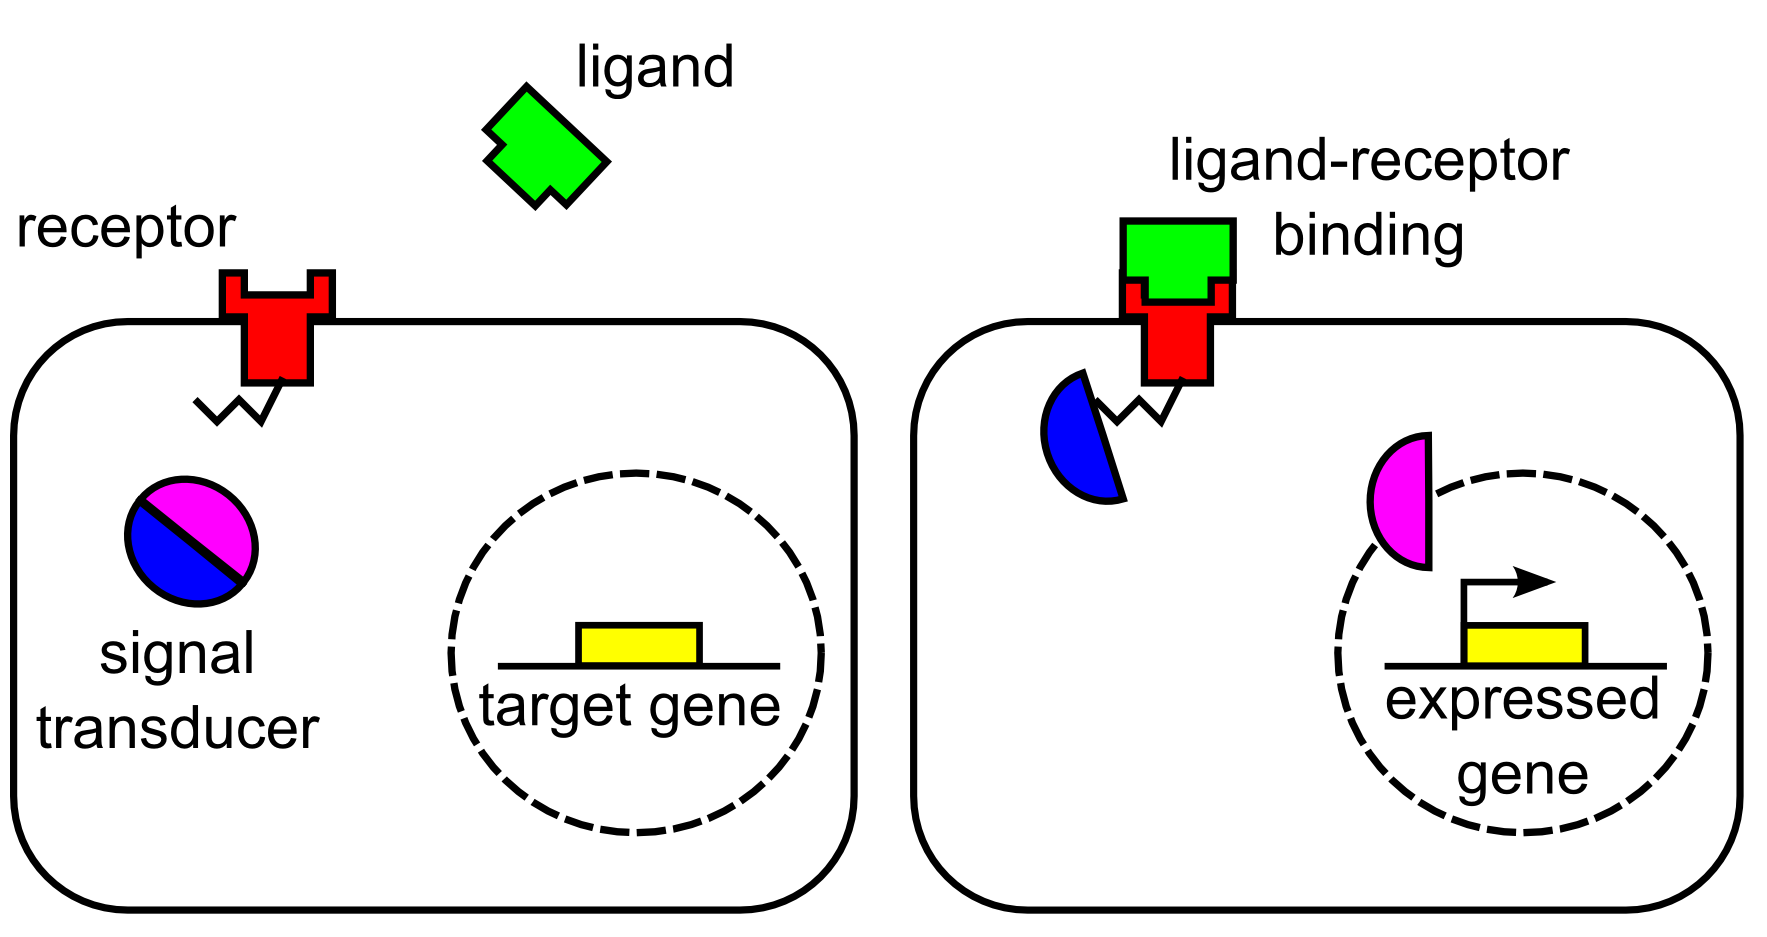
\includegraphics[width=10cm]{./Images/signalling.png}
%  \centering
%  \caption{
%  Scheme of an hypothetical signalling pathway. Left: The extracellular ligand (green) is not bound to the membrane receptor (red) so the signal transducer protein (blue/magenta) is inactivated. In the nucleus (dashed circle) the target gene (yellow box) is inactive. Right: As the ligand binds to the receptor, the cytoplasmic domain (depicted as a zigzag tail) of the receptor change to an active conformation, cleaving the signal transducer. Part of the signal transducer acts as a transcription factor, going into the nucleus where activates the transcription of the target gene after binding to its regulatory region.
% }
%  \label{fig:Signalling}
%\end{figure}
%%%%%%%%%%%%%%%%%%%%%%%%%%%%%%%%%%%%%%%%%%%%%%%%%%%%%%%%%%%%%%%%%%%%%%%%%%%%%%%%%%%%%%
%
%\paragraph{Transcription factors} The transcription factors (TFs) are proteins that bind to specific regulatory regions, to induce or repress the expression of a gene.
%Based on the secondary structure of the protein binding domain, TFs can b e classified in four main families: helix-turn-helix, helix-loop-helix, zinc finger and leucine zipper (\citep{Carroll2001}.
%	\nomenclature{TF}{Transcription Factor}
%	
%The members of each family has been recognised in playing different roles in development. For example, it has been observed that in diverse metazoan species C2H2 zinc-figers TFs are over-represented in early development, as opposite to Homeobox TFs which are under-represented in the same period \citep{Schep2013}.
%Hox genes (a subset of the Homeobox TF family) are involved in the A/P patterning of many metazoan groups. Intriguingly, these genes were found to have spatial collinearity in mice and flies (REF). That means that the A/P expression of the Hox genes reflects their physical order along the chromosome.
%At the time of its discovery, collinearity of Hox genes were considered as a master plan for A/P patterning in animals (REF).
%However, after Hox genes were investigated in more species it became clear that in some species with Hox genes collinearity is not always present, and some species do not have Hox genes at all (REF).
%
%\paragraph{Signalling pathway genes} Signalling pathways are usually a complex network of molecules including extracellular diffusible signals, membrane receptors, intermediate signal transducer molecules and transcription factors.
%Signalling pathways usually begin with a extracellular signal that causes a conformational change in its cell membrane receptor after binding to it.
%The new conformation results in enzymatic activity in the cytoplasmic domains of the receptor protein, that phosphorylate other cytoplasmic proteins.
%Finally, one or more activated transcription factors induce or repress specific gene activity \citep{Gilbert2014}.
%
%Signalling pathways recurrently used during animal development are the Wnt, FGF and Shh pathways (for a detailed description of each signalling pathway, see \citep{Gilbert2014}.
%For example, the Shh pathway plays a fundamental role in the fruit fly segment polarization(REF) and wing development (REF), and in vertebrate limb (REF) and tooth development \citep{Jernvall2000b}.

\subsection{Spatial complexity}

Until this point, I have focused on the concept of compartmentalization 
%(and the molecular regulatory mechanisms that might be responsible for it) 
as one aspect that reflects the increase in complexity during development.
Another aspect that is intuitively related to the increasing embryonic complexity is the shape (or form) of the embryo. Focusing on the shape of the embryo, embryonic development can be thought as a process that starts with a simple spherical or oblate fertilized egg and that ends with complex shapes and forms (in the adult or larva) \citep{Forgacs_Newman2005}.

\subsubsection{Morphometrics}

In the last decades, morphometric tools have been used widely as a tool to quantify, characterize and compare biological shapes \citep{JamesRohlf1993}. In morphometrics, shape refers to the geometric properties of an object that are invariant to location, scale and orientation \citep{Slice2005}. Many of the modern morphometrics analyses are based on the use of "landmarks", which refer to precisely located points that establish a clear one-to-one correspondence between the samples under study \citep{Klingenberg2010}. Although there are many different morphometric methods, they can be divided in four main categories: "traditional morphometrics", "geometric morphometrics", outline analysis and surface analysis \citep{Slice2005}. In the next paragraphs I will briefly explain these different methods. For an extensive review, see \citep{Bookstein1997,Dryden1998,Zelditch2008,Slice2005}.

The "traditional" methods refer to the application of multivariate statistics (e.g., principal component analysis) to the direct measurement of lengths, widths or ratios of specific structures. Some typical applications of these methods were the classification of species or sexes \citep{Jolicoeur1960} using lentghs, widths or anlges between landmarks \citep{Dryden1998}.

Geometric morphometrics analyses use instead geometric coordinates of morphological landmarks \citep{zelditch2012geometric}. 

Outline analyses are specially relevant when it is not possible to identify comparable landmarks between samples. 


Uses Fourier decomposition to produce "harmonics" that describe the positions of the points along the outline. The harmonics can be converted into shape coordinates and ultimately into principal components.

 semilandmarks are the points along a curve. If strategically spaced, they can be submitted to Procrustes analysis and analyzed just like ordinary landmarks.
Sliding semilandmarks - The position of semilandmarks can be optimized by sliding them along the outline curve as part of Procrustes analysis to provide the best fit between shapes. 

\subparagraph{Eigenshape and extendend eigenshape analysis} 
Eigenshape analyses use a different approach to outline coordinates where the standardization is not done with Procrustes, but by calculating angles between points to provide map around the curve. Principal components scores are derived from the angular data. Extended eigenshape analysis - Same as eigenshape, but a series of homologous landmarks are used to pin the outline at points along the perimeter
of an object.



\paragraph{Surface analyses}

%
%\subsection{Analysis of gene expression as a proxy of compartmentalization and complexity in the embryo}
%
%SEARCH FOR EXAMPLES THAT ARE SIMILAR TO MY STUDY, AND THAT CAN BE USED AS A PROXY OF COMPARTMENTALIZATION 
%
